\section{Introduction} \label{introduction}
This thesis aims to be an introduction into volume rendering data structures as well as introduce two compression steps of volume density data. The focus is not so much on shrinking our geometry, but more so shrinking the actual density data. This is required for our desire to implement full three-dimensional volume animation models in the in house renderer at Traverse Research. A basic understanding of the Graphics processing unit (GPU) is expected. Along with knowledge of the basic terminology used when talking about ray tracing such as acceleration structures, primitives, rays and the rendering equation.


\subsection{Traverse Research} \label{introduction:traverse_research}
\href{https://traverseresearch.nl/}{Traverse Research} is a company which does state-of-the-art research in graphics, and more specifically ray tracing. Traverse does research for multiple hardware vendors including AMD and ARM, for whom they develop ray tracing algorithms, optimizations and workloads.
\subsubsection{Breda} \label{introduction:traverse_research:breda}
Traverse's current in-house hybrid rendering framework "Breda" includes many features which are expected from a modern renderer. However, volume rendering is still largely unexplored. Breda can compile for either a Vulkan or DirectX 12 backend to make use of the latest ray tracing features. Along with that, some advanced rendering techniques are used. Most notably bindless rendering\cite{BindlessRenderingSetup} and render graphs\cite{RenderGraph101}. The former is a different way of interfacing with data on the GPU, while the latter simplifies GPU synchronization while optimizing dispatch ordering based on read and write dependencies of different pieces of data on the GPU. All of this is written in Rust and HLSL.
\subsubsection{Volumes} \label{introduction:traverse_research:volumes}
In parallel to this research there is another project going on which focuses on shading as explained in Section \ref{related_work:path_traced_volume_rendering}. The combination of both projects allows for physically based shading of large animated volumetric effects in real time. The exact placement of this research inside the Breda framework can be seen in Figure \ref{fig:project_structure}.

\begin{figure}[H]
    \centering
    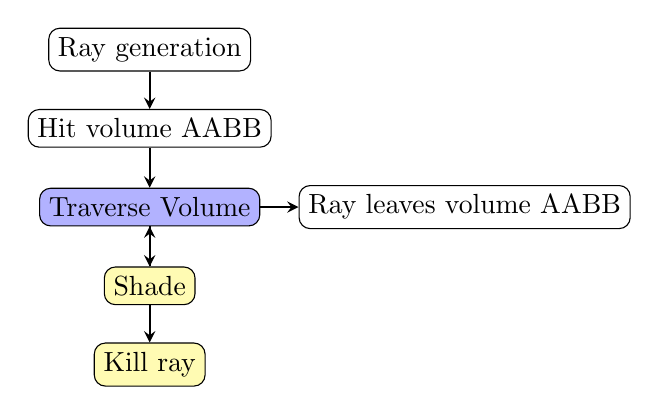
\begin{tikzpicture}[node distance=1cm]
        \tikzstyle{arrow} = [thick,->,>=stealth]
        \tikzstyle{done} = [rectangle, rounded corners, minimum width=1cm, minimum height=0.33cm,text centered, draw=black]
        \tikzstyle{this} = [rectangle, rounded corners, minimum width=1cm, minimum height=0.33cm,text centered, draw=black, fill=blue!30]
        \tikzstyle{other} = [rectangle, rounded corners, minimum width=1cm, minimum height=0.33cm,text centered, draw=black, fill=yellow!30]
        \node (start) [done] {Ray generation};
        \node (aabb) [done, below of=start] {Hit volume AABB};
        \node (trav) [this, below of=aabb] {Traverse Volume};
        \node (shade) [other, below of=trav] {Shade};
        \node (kill) [other, below of=shade] {Kill ray};
        \node (leaves) [done, right of=trav, xshift=3cm] {Ray leaves volume AABB};

        \draw [arrow] (start) -- (aabb);
        \draw [arrow] (aabb) -- (trav);
        \draw [arrow] (trav) -- (shade);
        \draw [arrow] (trav) -- (leaves);
        \draw [arrow] (shade) -- (trav);
        \draw [arrow] (shade) -- (kill);

    \end{tikzpicture}
    \caption{Flow diagram highlighting where this research fits inside the Breda framework. The white boxes indicate parts of the pipeline which already exist inside the Breda framework. The blue box shows what this research will focus on, and the yellow boxes highlight what parts were developed in parallel to this research. As can be seen, when rays bounce inside a volume, they can repeatedly be shaded and continue traversal until they either leave the volume or are killed because they won't contribute any light to the scene.}
    \label{fig:project_structure}
\end{figure}